\chapter{Evaluation}
\label{chap:evaluation}
We implemented the algorithm explained in Chapter \ref{chap:testgeneration} in an Eclipse plug--in and successfully tested it for a set of academic problems and performed a case study with a real world model from Airbus. We will point out that the transparent interchangeability of solvers is indeed one of the biggest advantages of the approach presented in this thesis. Also the limitations as well as missing but easily implementable features will be discussed in Section \ref{sec:evaluationLimitations}.
\section{Example Models and Case Study}
In order to demonstrate the strength of our approach we built a set of test models. Each test model corresponds to one of the mathematical programming problems presented in the \nameref{chap:preliminaries} Section \ref{sec:Maths}. For each model we selected a suitable solver to generate the necessary test data. 

We also build a C-implementation for each academic test model and 
\subsection{Different Constraint Types and their Handling}
\label{sec:evaluationAcademicModels}
We will start with models, which require easy problems to be solved in order to obtain test data. By easy we mean decidable problems with a tractable algorithm. Then we will explain how we generated test data for problems, which require either non trivial problems to be solved. We consider problems with intractable algorithms as non trivial. Finally we will also present models, which require an instance of an undecidable problem to be solved in order to obtain test data. That means we can only generate test data for them with tractable or intractable heuristic methods.\\
Each solver is suitable for another problem class and for several problem classes there are multiple solvers that could be used. We performed some comparisons of different solvers in terms of runtime and the test data produced. For each presented test model we produced test data for all paths up to some maximum length and examined how much more effort in terms of runtime it is to generate boundary values as test data.\\
Finally we built a C implementation of the function modelled by the input to our algorithm and execute the generated test suite against this implementation. We also manually introduced some errors into the implementation and verified, that the produced test suite contains test cases that fail on those errors and that all test pass when the implementation is correct.
\subsubsection{Linear}
\paragraph{Pure Floating Point Variables}
\paragraph{Mixed Integer}
solve with cplex up to 100000 Variables possible
\subsubsection{Non linear convex}
solvable with every Solver implementing some version of Newton Algorithm on Sparse Matrices like Minos, Knitro or Quadratic programming approaches like in CPLEX.
\subsubsection{Non Convex}
\label{sec:exampleModelNonConvex}
\begin{figure}
\label{fig:pumpTyre}
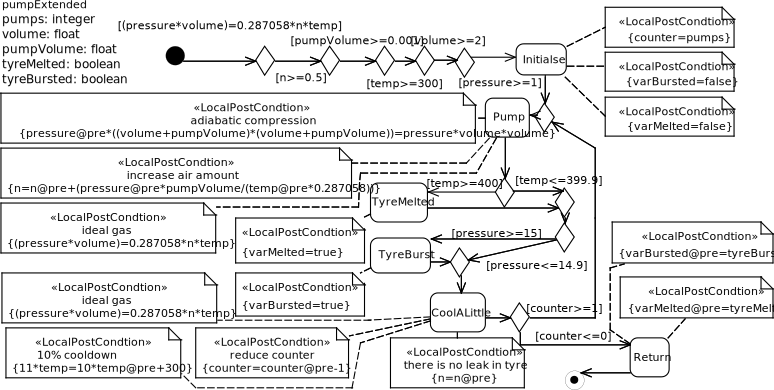
\includegraphics[width=\textwidth]{./pics/pumpTyre.pdf}
\caption{Activity Diagram with non convex mixed integer constraints}
\end{figure}
in general undecidable couenne finds solutions sometimes.
The Example Model here is the Exploding Tyre Model
\subsubsection{Constraint Programming}
ILOGCP, Gecode or transformation possible
\paragraph{Integer arithmetic only} Gecode
\paragraph{linear mixed Integer arithmetic} IlogCP
\begin{figure}
\label{fig:classifyTriangle}
\includegraphics[width=\textwidth]{./pics/TriangleClassificator.pdf}
\caption{Activity Diagram with non convex mixed integer constraints}
\end{figure}
\paragraph{nonlinear mixed Integer arithmetic}
really really really problematic. Currently the only way is to transform the Activity Test Case Graph to remove the Logical Operations in favour of parallel or sequential Control Flows with guards. Use COUENNE.
\subsection{Case Study PAX Model}
\label{sec:evaluationCaseStudy}
We tested our implementation on a model modelling the PAX call system from Airbus. Out of the model of the complete product we selected an activity diagram modelling the interaction of the PAX call system with the \textbf{I}n \textbf{F}light \textbf{E}ntertainment (IFE) system. The selected \UMLType{Activity} contains 21 \UMLType{Actions}, 24 \UMLType{ControllNodes}, and two \UMLType{LoopNodes}. Furthermore there are eight \UMLType{DataStoreNodes} representing function local variables. The model was originally created with Artisan Studio, and used to generate a C-implementation from it with a proprietary code generator from Atego\textsuperscript{\textregistered}. The branching conditions and the code body of each \UMLType{Action} is given in C--syntax. All assignments and conditions consist of linear equations and inequalities only; thus the constraint satisfaction problem to be solved for test data generation is a linear program.\\
The described algorithm has several parameters, which mainly influence the \nameref{sec:pathsearch}. We use this case study to evaluate the influence of those parameters on the runtime of the Algorithm. The examined parameters are the maximum length of control flow paths to be tested, the maximum amount of test cases to be generated, and the frequency at which the early infeasible path check is performed during the path search.
\subsubsection{Manual Adaptation}
In order to generate C++ unit test code with our Eclipse plug-in from the described model several pre-processing steps need to be performed manually. Those manually to perform steps are the conversion of the Model from Atego\textsuperscript{\textregistered } Artisan Studio into Eclipse UML, adding all constraints in OCL syntax, the guards and the local post--conditions, flattening the \UMLType{LoopNodes}, and replacing the \UMLType{DataStoreNodes} by \UMLType{Properties}.\\
Atego\textsuperscript{\textregistered} does not store models natively in xmi format but has an option for exporting models in xmi format. The Eclipse Modelling Framework natively uses the xmi format to store models. Each modelling tool uses its own implementation of the UML meta model and there are slight differences in the implementations making the created models incompatible with each other. In order to import the model from Artisan in Eclipse we manually need to remove some objects not recognised by Eclipse and correct some typing errors in the xmi file. Then we can load the XMI and browse the model with the Eclipse Modelling Framework.\\
Every \UMLType{Action} is associated with a C-code snippet that is used for code generation. There are not yet \UMLType{Constraints} specifying the pre and post--conditions of each \UMLType{Action} in OCL. Also the \UMLReference{guards} do not contain OCL queries. We make an educated guess to add \UMLReference{guards} and \UMLReference{localPostconditions} reproducing the semantics of the C-code snippets contained in the original model. The original model used local C-struct variables modelled by the \UMLType{DataStoreNodes} contained by the \UMLType{Activity}. Our implementation can handle primitive data type variables modelled by \UMLType{Properties}, consequently we created one \UMLType{Property} per field of a struct variable. The original model also used arrays. We emulated the behaviour of an indexed collection by allowing all variables depending on an index to change to an arbitrary value whenever the index is changed. This may produce wrong behaviour but seemed fair enough to evaluate our algorithm. The \UMLType{DataStoreNodes} will be ignored by our algorithm.\\
The \UMLType{LoopNodes} contain further model elements in their \UMLReference{bodyPart} reference. Those elements from the \UMLReference{bodyPart} are directly included into the parent \UMLType{Activity} the \UMLType{InitialNode} and \UMLType{FinalNodes} of the loop body are replaced by decision nodes and directly connected to every element that was connected to the \UMLType{LoopNode}. In order to preserve the loop semantic a control flow from every final node of the body to the initial node of the body is added and decorated with a \UMLReference{guard}.\\
The function specifying which control flow to take after each \UMLType{Action} is \emph{well--defined} and \emph{defined} over the complete domain. Well--defined means there is no possible state in which more than one guard evaluates to true, and defined over the complete domain means that there is no value assignment for which all guards of the outgoing \UMLType{ControlFlows} evaluate to false.
\subsubsection{Runtime Experiments}
\begin{figure}
\begin{tikzpicture}
\begin{axis}[
width=0.49\textwidth,
ymajorgrids=true,
yminorgrids=true,
xmajorgrids=true,
no markers,
ymode=log,
]
\addplot table[x=Max_PATHLENGTH,y=ElapsedTime(ns)]{Experiment-DATA/RuntimeExperimentCaseStudy.txt};
\addplot table[x=PATHSEARCH_MAX_PATHLENGTH,y=time(ns);]{Experiment-DATA/Runtime10-100.txt};
\addplot table[x=PATHSEARCH_MAX_PATHLENGTH,y=time(ns)]{Experiment-DATA/Runtime210-80.txt};
\addplot table[x=Max_PATHLENGTH,y=ElapsedTime(ns)]{Experiment-DATA/RuntimeExperimentCaseStudy2.txt};
\end{axis}
\end{tikzpicture}%
\begin{tikzpicture}
\begin{axis}[
width=0.49\textwidth,
ymajorgrids=true,
yminorgrids=true,
xmajorgrids=true,
no markers,
ymode=log,
] 
\addplot table[x=PATHSEARCH_UNCHECKED_STEPS,y=time(ns);]{Experiment-DATA/RuntimeExperimentUncheckedPaths.txt};
%\addlegendentry{Max_Pathlength = 40}
\addplot table[x=PATHSEARCH_UNCHECKED_STEPS,y=time(ns);]{Experiment-DATA/RuntimeExperimentUncheckedPaths2.txt};
%\addlegendentry{Max_Pathlength = 50}
\addplot table[x=PATHSEARCH_UNCHECKED_STEPS,y=time(ns);]{Experiment-DATA/RuntimeExperimentUncheckedPaths2.txt};
%\addlegendentry{Max_Pathlength = 50}
\addplot table[x=PATHSEARCH_UNCHECKED_STEPS,y=time(ns);]{Experiment-DATA/RuntimeExpPathlength60.txt};
\addplot table[x=PATHSEARCH_UNCHECKED_STEPS,y=time(ns);]{Experiment-DATA/RuntimeExpPathlength70.txt};
\addplot table[x=PATHSEARCH_UNCHECKED_STEPS,y=time(ns);]{Experiment-DATA/RuntimeExpPathlength80.txt};
%\addlegendentry{Max_Pathlength = 60}
\end{axis}
\end{tikzpicture}%
%\end{center}
\caption{Runtime of Test Generation }
\label{fig:RuntimeExperiments}
\end{figure}
The implemented algorithm has several properties influencing the exact execution of the \nameref{sec:pathsearch}. In this section we will examine the influence of these parameters on the number of unit tests generated and the runtime of the algorithm. As already explained in Section \ref{sec:pathsearch} and Section \ref{sec:EarlyInfeasiblePathRecognition} there are two parameters that ensure the termination of the \nameref{sec:pathsearch}. Those are the maximal pathlength and the maximum amount of test cases generated. It is quite obvious that the number of test cases found may depend exponentially on the maximal control flow path length. We assume, that the path search algorithm described in Section \ref{sec:pathsearchDFS} will find abstract test cases at a constant rate. According to this assumption the runtime of the algorithm should linarly depend on the amount of test cases generated. Thus the maximal number of test cases to be found should be correlated linearly to the overall runtime of the algorithm, and we expect the maximum control flow path length to be exponentially correlated to the runtime of the test generation algorithm. \\
There is also one parameter steering the early infeasible path elimination. That is the amount of unchecked steps. Calling the solver is verry expensive in terms of runtime. To check wheather the current control flow path is infeasible we need to solve the corresponding constraint satisfaction problem. If we check everytime one control flow has been added to a control flow path we will eliminate infeasible paths as soon as possible, but will also call the solver unecessaryly often to find out that one constraint added did not make the path infeasible. If we perform a check for infeasible control flow paths after every tenth decision passed we will have to check at least $2^10$ control flow paths wheather they are feasible or not, where several of them could have been eliminated much earlier by computing much less constraint satisfaction problems. We pay special interrest to the influence of the number of unchecked decissions before control flow paths are checked for feasiblility. We assume, that there will be a minimum of runtime for some number of unchecked decissions.

%Complex data types we added one \UMLType{Property} per field in a variable.

%When the Model was correctly imported we need to add to each \UMLType{Action} those local post--conditions that describes the assignments done in the C-code associated with that \UMLType{Action}



I could do a case study with the Airbus PAX call model from Atego\textsuperscript{\textregistered }.
\section{Verification of the Implementation}
We claim that the Eclipse plug--in built aside this thesis implements the algorithm explained in \nameref{chap:testgeneration}. This claim is validated manually by checking each step separately. We use the Academic Example models presented in Section \ref{sec:evaluationAcademicModels} as test cases to verify each transformation described in \nameref{chap:testgeneration}. From each input model we created manually the intermediate artefacts that should have been created according to the specification and compared them to the intermediate artefacts produced by the plug-in.
\section{Limitations}
\label{sec:evaluationLimitations}
\subsection{Theoretical Limitations}
undecidability of nonlinear arithmetic over infite sets and Exponential runtime for Constraint solving algorithms for some formulations
\subsection{Limitations of the Implementation}
no structured activity nodes, no invariants, not completely implemented test goal management.
\subsection{Limitations of used Tools}
XMI interchange format does not work always LOTS OF BUGS!!!!
\subsubsection{AMPL}
\label{sec:LimitationsAMPL}
\section{further Ideas}
There is no good reason for using OCL as the specification language in order to ease the constraint solving prolog could directly be used as language to specify constraints in a UML Model.


